%%%%%%%%%%%%%%%%%%%%%%%%%%%%%%%%%%%%%%%%%%%%%%
\logvartrue
\chapter{A life in transition: bacteria in harsh environments}
%%%%%%%%%%%%%%%%%%%%%%%%%%%%%%%%%%%%%%%%%%%%%%
Bacteria are everywhere and they make up for their small dimensions in sheer number. Thanks to their flexible metabolism, bacteria have been able to thrive in almost all environments on the heart, from acid mines to sulphur pools. However, studying bacterial communities in such environments can be very difficult since, as said, only a small fraction of bacteria can be isolated under standard laboratory conditions. Indeed, it is estimated that in a single gram of soil live more than 4000 different bacterial ``genomic units'' based on DNA - DNA re-association studies, but only less than 1\% of this immense diversity can be isolated and cultured. To overcome the limitations imposed by existing laboratory techniques, many future efforts should be directed  toward sequencing of environmental DNA in order to extract all genetic informations contained in the environment. For this reason we have focused our attention to the study of bacterial communities in harsh environments using sequence-driven approaches based on the 16S rRNA gene sequences. This approach has allow us to retrieve informations about microbial populations not otherwise obtainable with standard microbiology techniques.\\
These topics have been discussed in the following published papers:\\
\vspace{-5mm}
\begin{itemize}[nosep]
\item \textbf{Bacci, G.}, Pagoto, E., Passaponti, M., Vannocci, P., Ugolini, A., \& Mengoni, A. (2014). Composition of supralittoral sediments bacterial communities in a Mediterranean island. \textit{Annals of Microbiology}, 1-13.\\
\item Borruso, L., \textbf{Bacci, G.}, Mengoni, A., De Philippis, R., \& Brusetti, L. (2014). Rhizosphere effect and salinity competing to shape microbial communities in \textit{Phragmites australis} (Cav.) Trin. ex-Steud. \textit{FEMS microbiology letters}, 359(2), 193-200.\\
\item Canfora, L., \textbf{Bacci, G.}, Pinzari, F., Papa, G. L., Dazzi, C., \& Benedetti, A. (2014). Salinity and bacterial diversity: to what extent does the concentration of salt affect the bacterial community in a saline soil?. \textit{PloS one}, 9(9), e106662.\\
\end{itemize}


\section{Composition of supralittoral sediments bacterial communities in a Mediterranean island}
Marine coasts are one of the most heterogeneous, but still understudied ecosystems. Despite their key importance as transition ecosystems between sea and land, their microbiological composition has still not been fully addressed. Here we describe the extant microbiota of three sandy beaches, at Favignana Island, Italy, using four different methods: Terminal-Restriction Fragment Length Polymorphism (T-RFLP), sequencing of 16S rRNA genes by Illumina-Solexa technology, functional genes detection and quantitative Real-Time PCR. Results showed that all the investigated beaches harbour a rich bacterial diversity, showing characteristic bacterial patterns both between different beaches and along the sea-to-land axis of the same beach.\\

\newpage
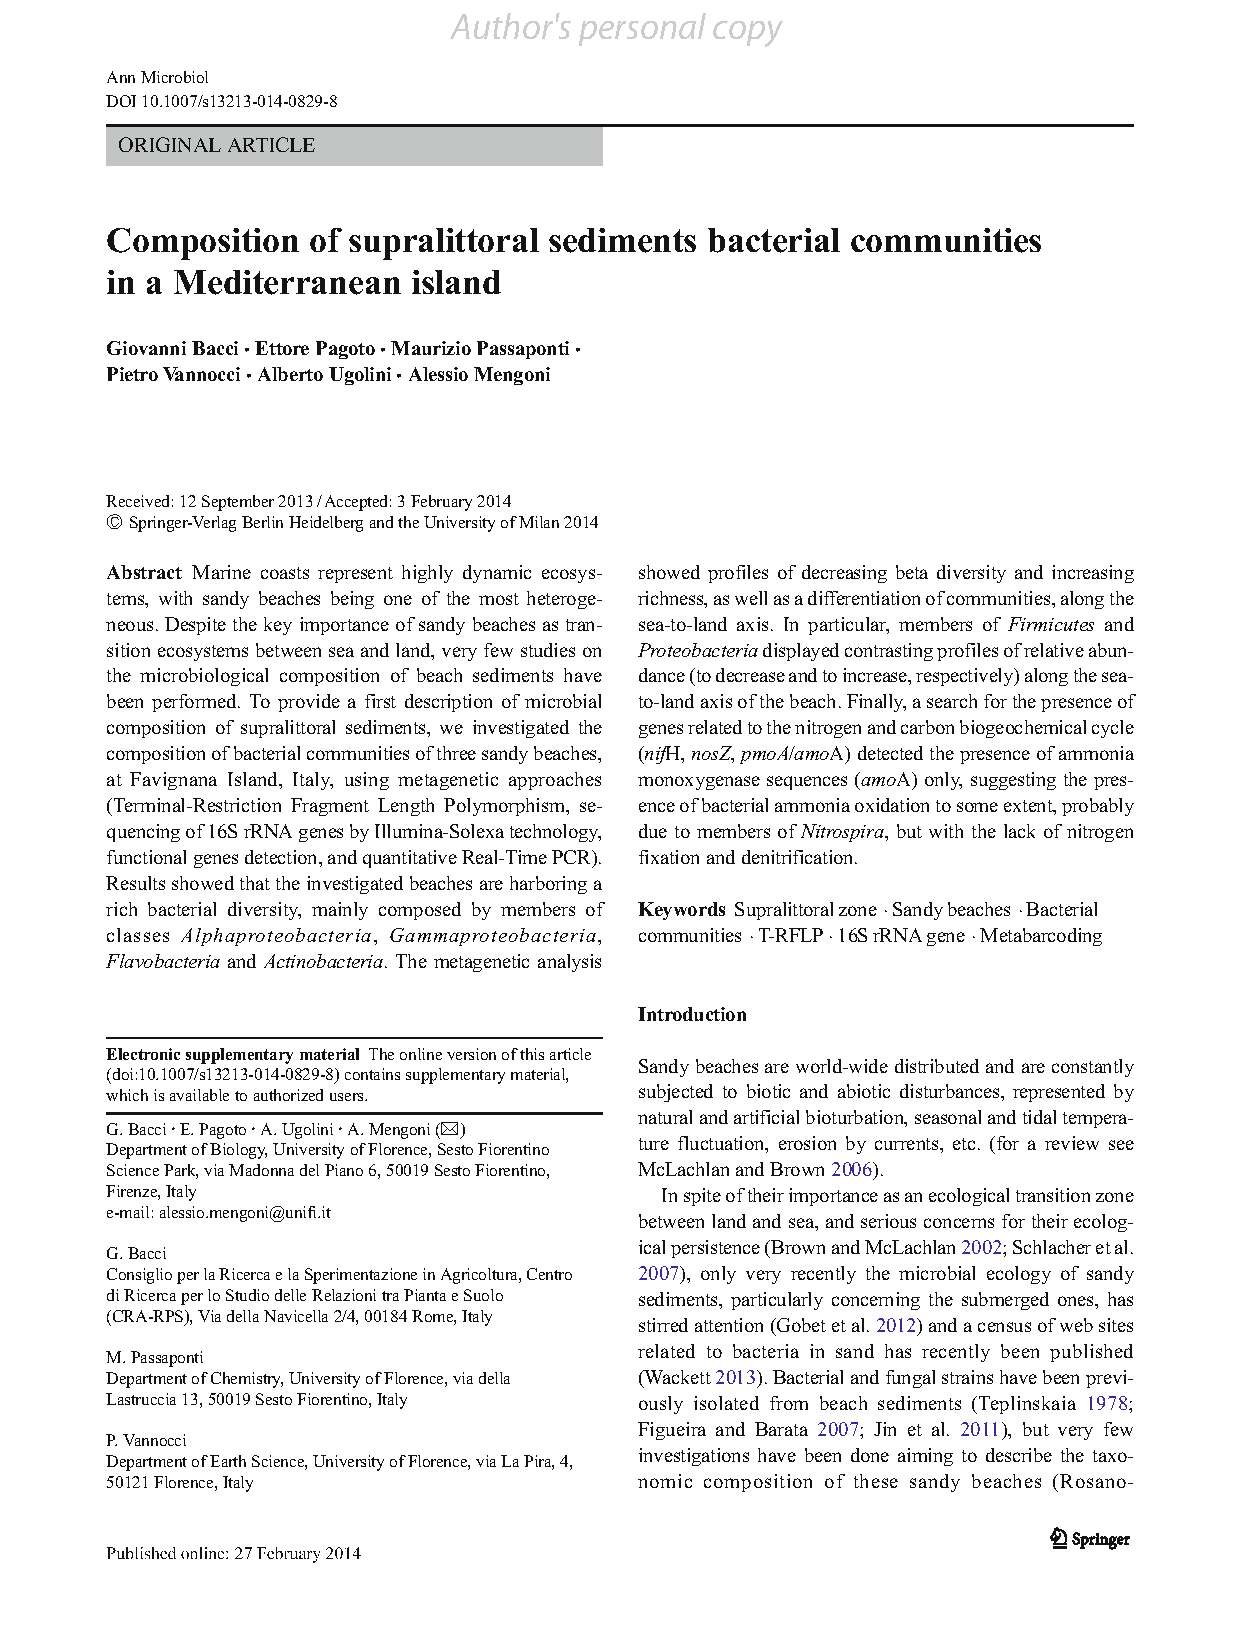
\includepdf[pages=-,offset=10mm 0, scale=0.9]{articles/favignana_mod.pdf}
\newpage

\section{Rhizosphere effect and salinity competing to shape microbial communities in Phragmites australis (Cav.) Trin. ex-Steud}
Hypersaline ecosystems are an example of extreme environments with salt concentrations approaching saturation. These regions are globally distributed both in marine and inland waters. Here, Rhizobacterial communities associated with Phragmites australis (Cav.) Trin. ex Steud. in a hypersaline pond close to Wuliangsuhai Lake (Inner Mongolia – China) were investigated and compared with the microbial communities in bulk sediments of the same pond. Rhizosphere samples showed an higher bacterial diversity compared to the bulk sediments, but the salinity levels appear to be the dominant factors able to shape bacterial patterns in the inspected samples.\\

\newpage
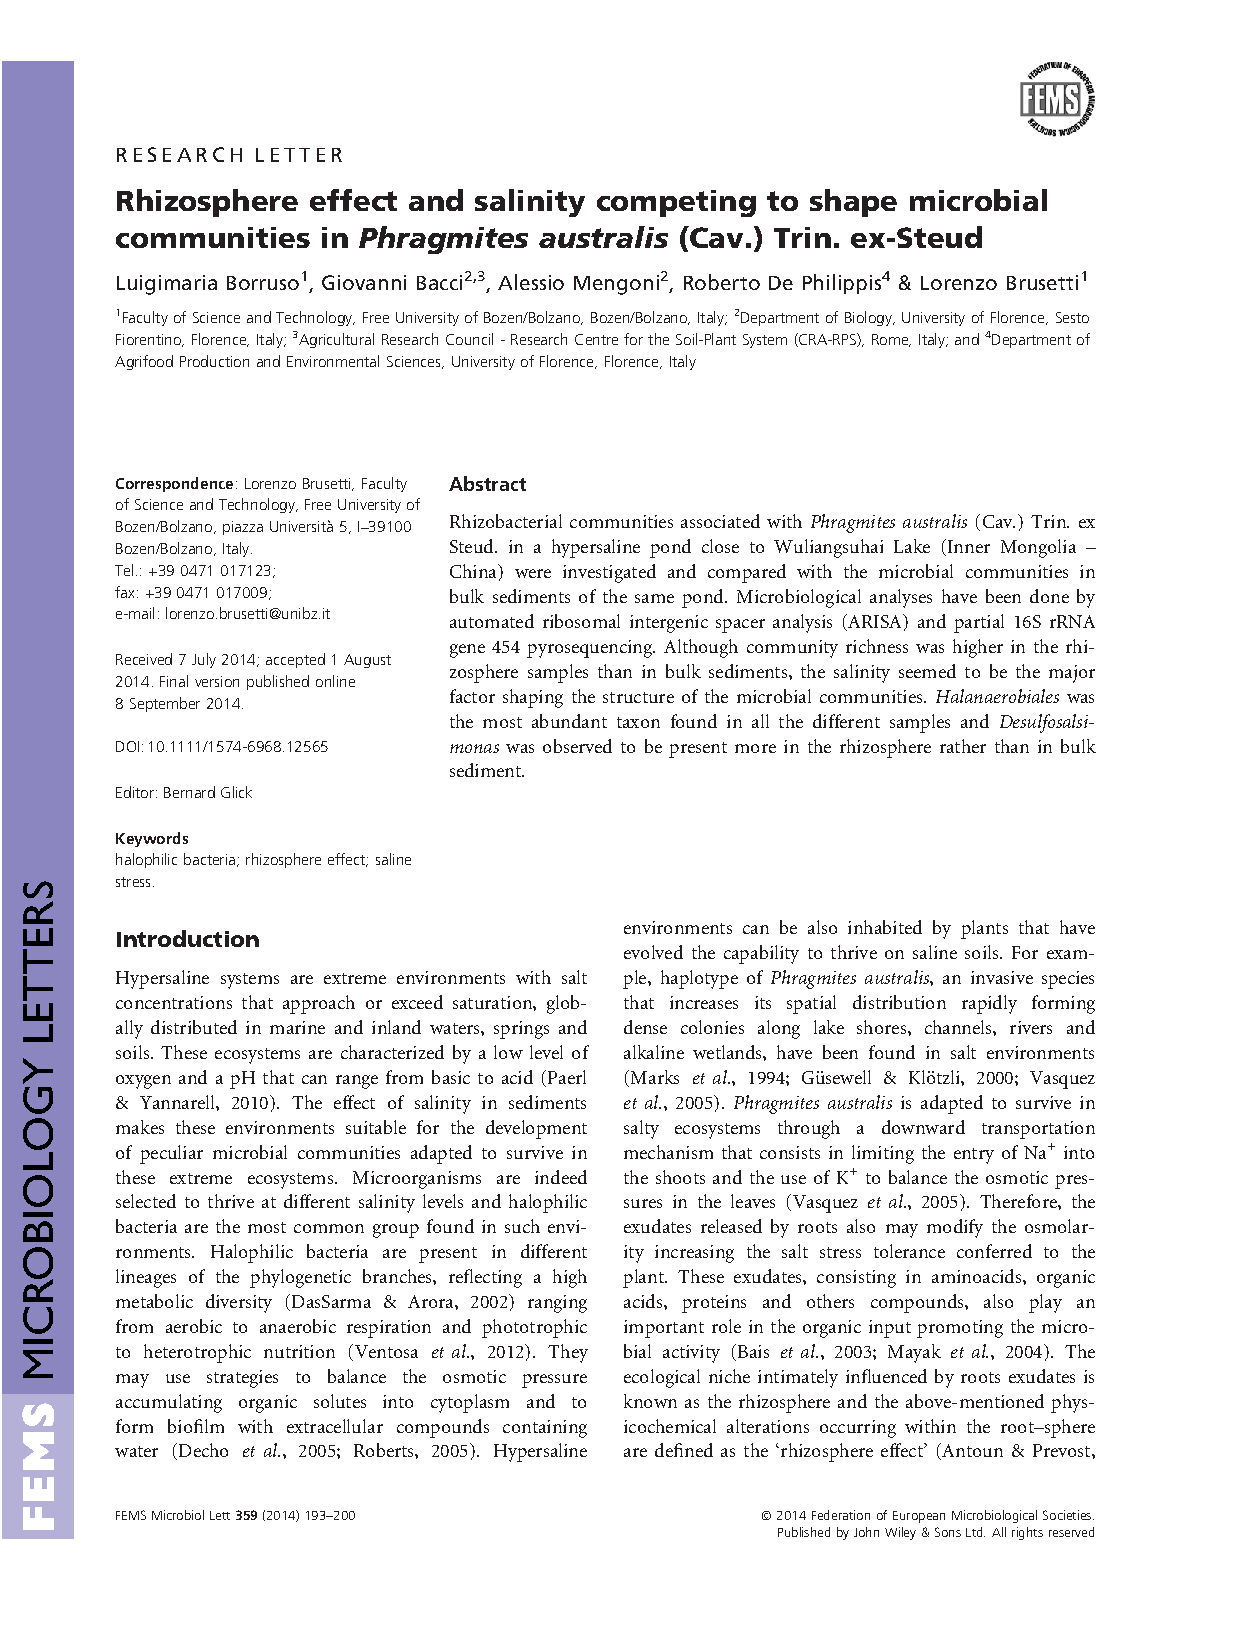
\includepdf[pages=-,offset=10mm 0, scale=0.9]{articles/borrusio.pdf}
\newpage

\section{Salinity and Bacterial Diversity: To What Extent Does the Concentration of Salt Affect the Bacterial Community in a Saline Soil?}
Salinization is a process able to increase the content of salt in a particular soil. This process can be caused even by natural processes (such as the gradual withdrawal of an ocean) or by artificial processes (such as irrigation). Here, soil characteristics were evaluated with a pyrosequencing analysis of two variable regions of the 16S rRNA gene (V2-V3) to deeply investigate the bacterial community structure in a natural saline soil located in Sicily (Italy). The aim of this study was to assess the organisation and diversity of microbial taxa using a spatial scale that revealed physical and chemical heterogeneity of the habitat under investigation.\\

\newpage
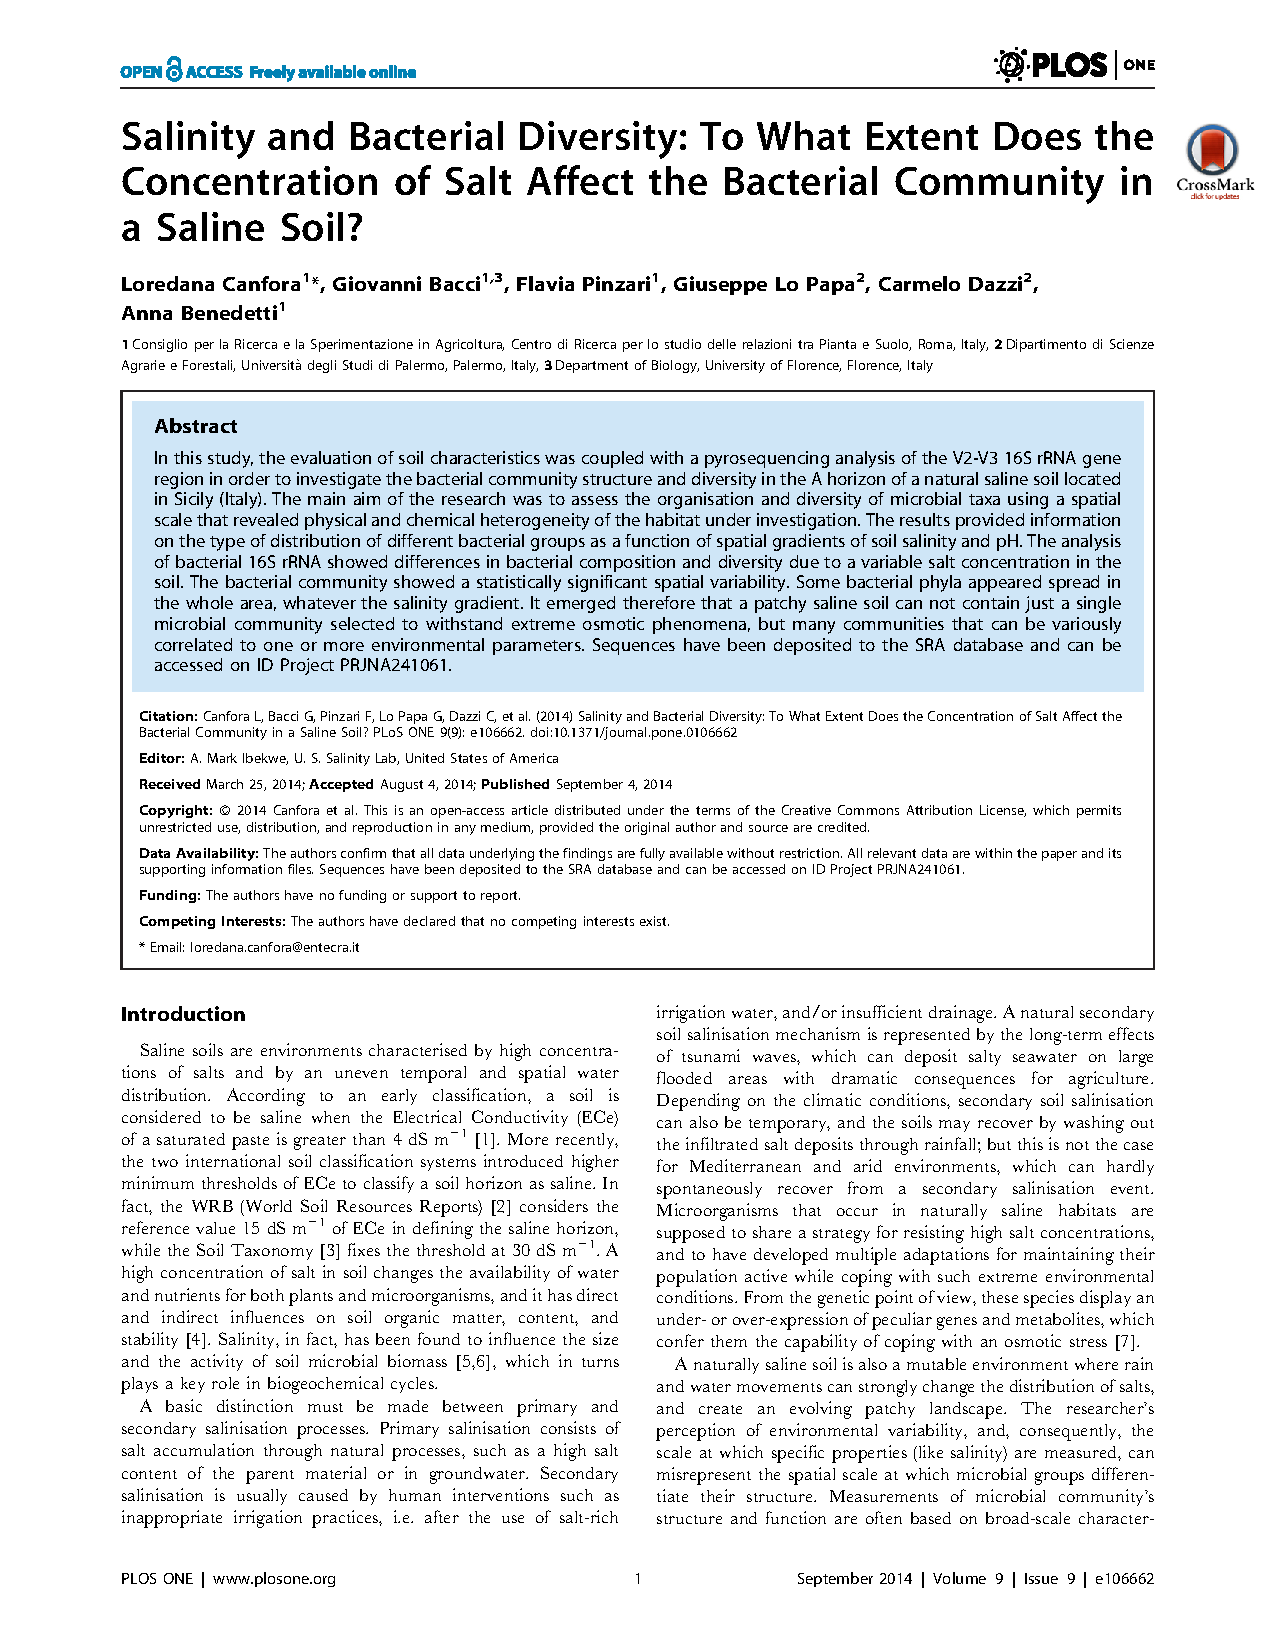
\includepdf[pages=-,offset=10mm 0, scale=0.9]{articles/loredana.pdf}
\newpage


%%-----------
%% Backmatter
%%-----------
\backmatter
\chaptermark{Bibliography}
\renewcommand{\sectionmark}[1]{\markright{#1}}
\bibliographystyle{unsrt}                           %Use alpha codes for references
\sectionmark{Bibliography}
\addcontentsline{toc}{chapter}{Bibliography}        %Force addition of Bibliography to TOC    
\bibliography{References}